%
% File acl2020.tex
%
%% Based on the style files for ACL 2020, which were
%% Based on the style files for ACL 2018, NAACL 2018/19, which were
%% Based on the style files for ACL-2015, with some improvements
%%  taken from the NAACL-2016 style
%% Based on the style files for ACL-2014, which were, in turn,
%% based on ACL-2013, ACL-2012, ACL-2011, ACL-2010, ACL-IJCNLP-2009,
%% EACL-2009, IJCNLP-2008...
%% Based on the style files for EACL 2006 by 
%%e.agirre@ehu.es or Sergi.Balari@uab.es
%% and that of ACL 08 by Joakim Nivre and Noah Smith

\documentclass[11pt,a4paper]{article}
\usepackage[hyperref]{acl2020}
%\usepackage{times}
\usepackage{latexsym}
\usepackage{graphicx}
\usepackage{xfrac}
\usepackage{mathtools}
\usepackage{amssymb}
\renewcommand{\UrlFont}{\ttfamily\small}


% This is not strictly necessary, and may be commented out,
% but it will improve the layout of the manuscript,
% and will typically save some space.
%\usepackage{microtype}
\aclfinalcopy

\title{Generating Knowledge Graphs from Large Language Models}

%\author{Yuri Kinakin \& David Noble}

\date{Jan 31, 2023}

\begin{document}

\maketitle
\section{Proposal}
Over last ten years, significant progress has been made on large language models for a wide variety of natural language processing tasks \cite{Min2021}. While these models can achieve (and even occasionally supersede) human level performance, they are significantly more internally complex than historical approaches. Simple explanations of what each model has learned make interpretation difficult, and as these models are expected to be applied against an increasingly wide variety of tasks, having the ability to easily query their internal logic is increasingly important. Some of this can be achieved through the use of a knowledge graph (KG), which encodes semantic information and provides a way to visualize contextual relationships \ref{KGfig}. Unfortunately, KGs have historically been complicated and onerous to create, requiring substantial manual input. A novel method to automatically generate KGs from a variety of large language models has been proposed by \cite{hao2022}. \par


We propose comparing KGs generated before and after a fine tuning exercise to help understand what is being learned by the model. Utilizing a domain-specific language corpus during fine tuning should help narrow the scope of changes. The Geological Survey of Canada has provided a series of notebooks to generate a machine readable corpus from their existing catalog of publications \cite{Raimondo2022}. We can then focus on a manual review of the major differences between the two KGs (before and after training) for geoscience specific words and concepts. \par

\begin{figure}
  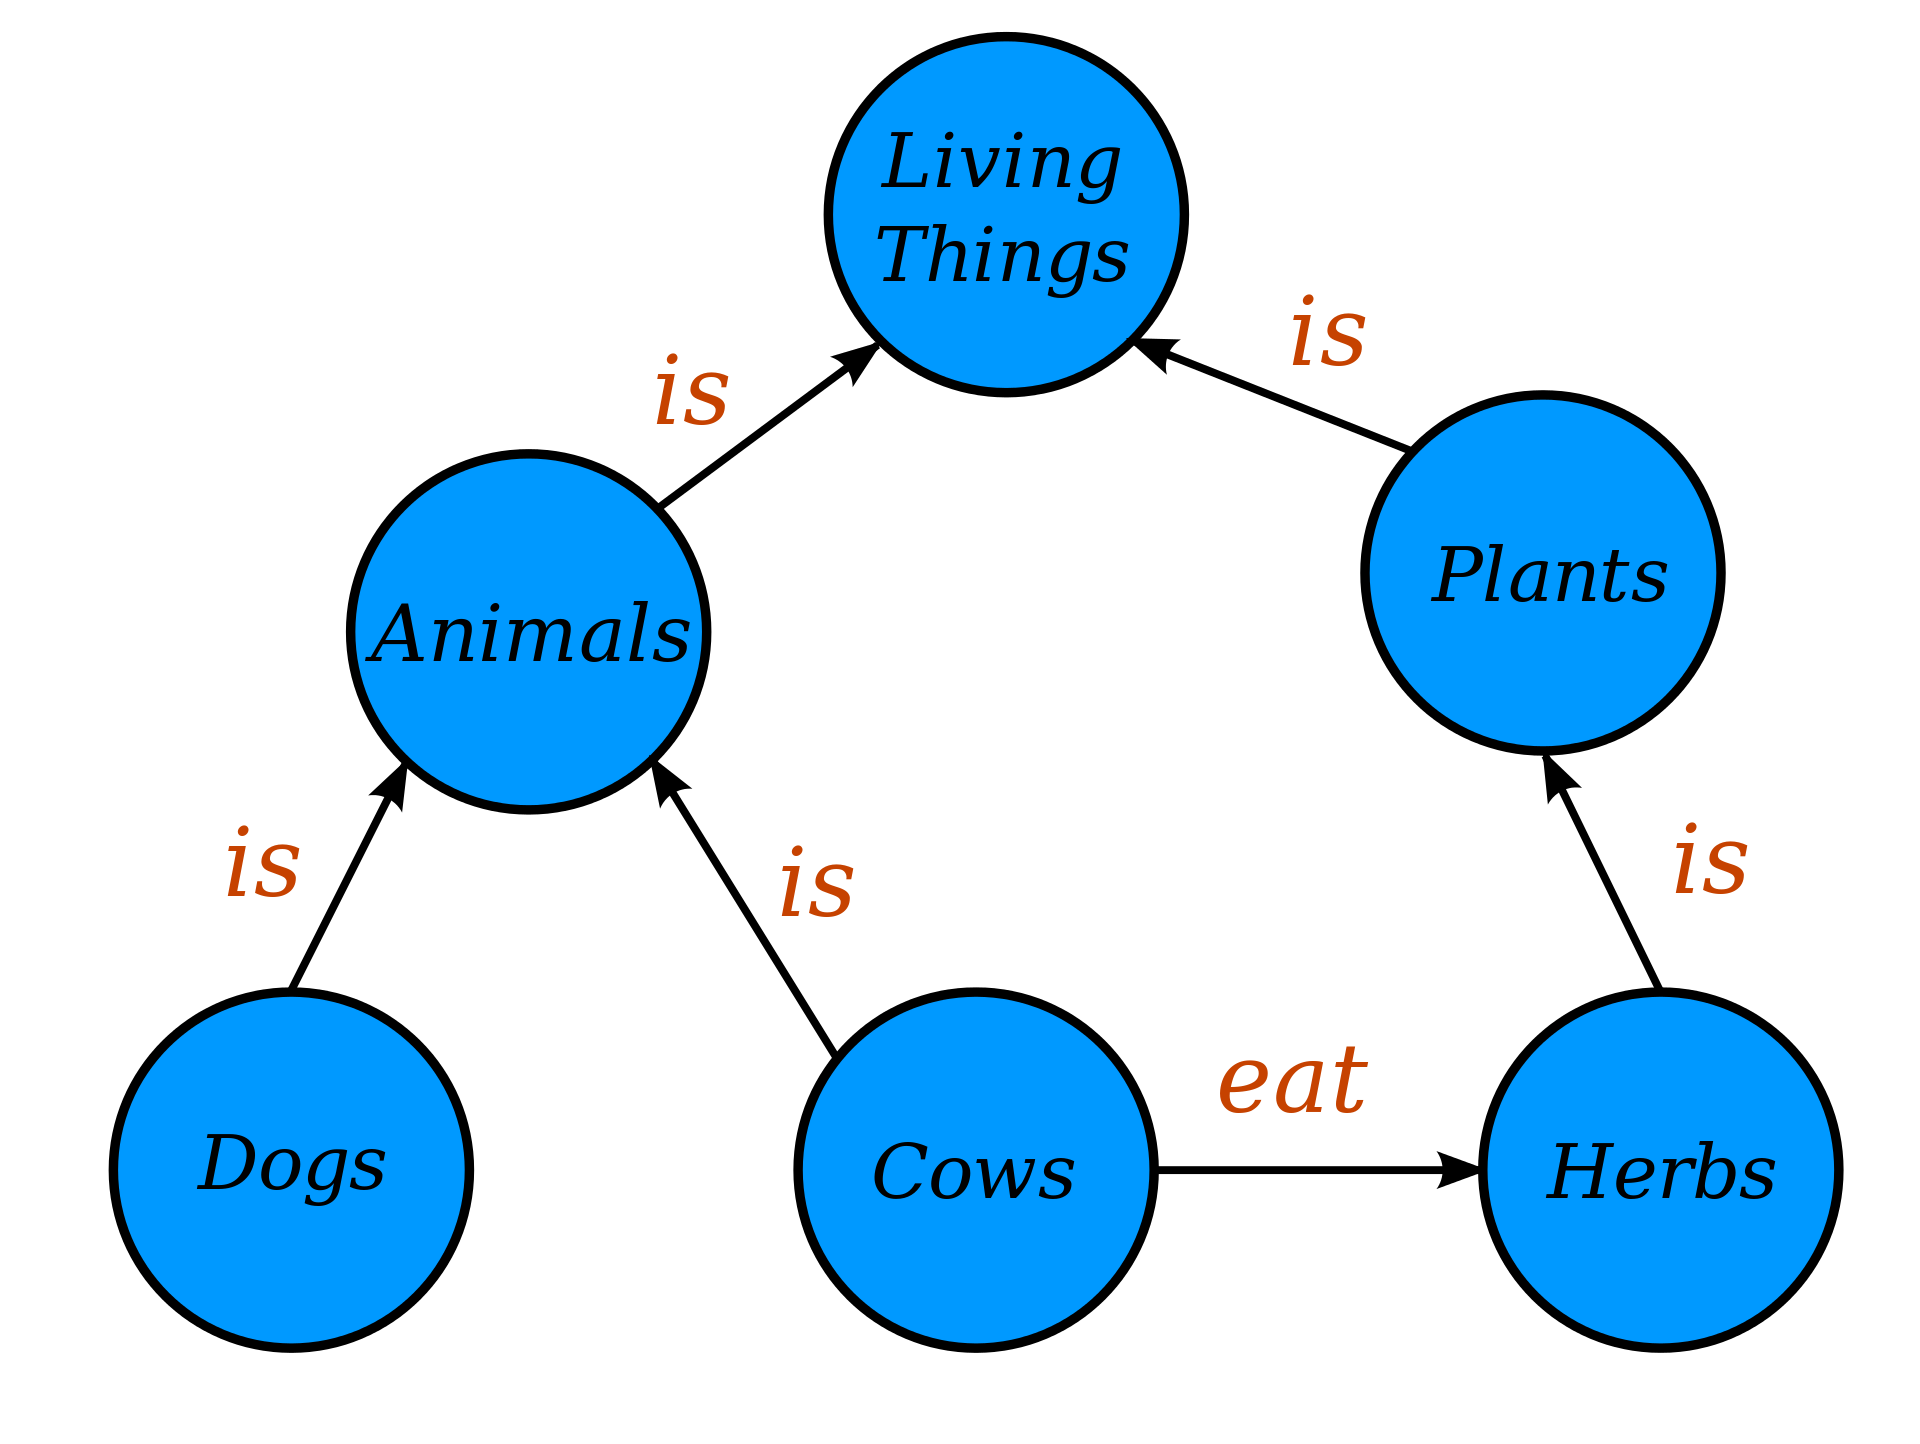
\includegraphics[width=\columnwidth]{KG}
  \caption{Example knowledge graph. \footnote{By Jayarathina - Own work, CC BY-SA 4.0, https://commons.wikimedia.org/w/index.php?curid=37135596.}}
  \label{KGfig}
\end{figure}

\bibliographystyle{apalike}
\bibliography{NLP}

\end{document}